%%%%%%%%%%%%%%%%%%%%%%%%%%%%%%%%%%%%%%
\chapter{Spectral Estimation}
%%%%%%%%%%%%%%%%%%%%%%%%%%%%%%%%%%%%%%

This chapter studies a very important estimation problem, which is that of estimating the power spectral density (PSD) of a stationary process. We will consider two families of estimators: 1) classical (or non-parametric) and parametric estimators, which are based on a model for the PSD.

Computing the estimate of $S_x(e^{j \omega})$, which we will denote by $\hat{S}_x(e^{j \omega})$, from an arbitrarily large number of realizations of a stationary process (see Figure \ref{fig:realizations_stochastic_process}) would be a (relatively) easy task. Of course, this is an idealized scenario as we do not have access to all realizations and, even more, we also do not have access to all time samples of the same realization. Thus, the objective in this section is to compute $\hat{S}_x(e^{j \omega})$ from $N$ samples of a single realization of the process $x[n]$.

The spectral estimation problem is defined only for wide-sense stationary (WSS) processes for which the mean function is time-independent, that is, $\mu_x = \mu_x[n] = \mathbb{E}[x[n]]$, and the auto-correlation function depends only on the time difference, i.e., $r_{x}[m] = r_{x}[n,n-m] = \mathbb{E}[x[n] x^{\ast}[n-m]]$. For non-stationary processes, the usual practice is to apply the estimators to small windows. That is, on a local scale we can assume that non-stationary processes are WSS. For instance, this is typically done when analyzing speech signals, which are usually described using non-stationary processes. Moreover, since only one realization is available, the process must be ergodic such that expectations can be substituted by time averages.

\begin{figure}
    \begin{center}
	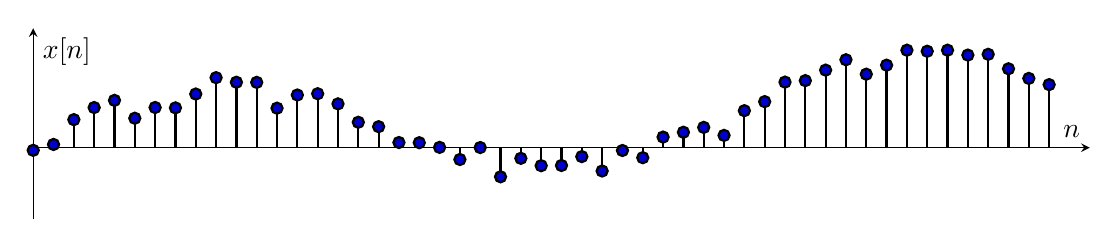
\begin{tikzpicture}
		\begin{axis}[%
		axis x line=middle,
		axis y line=middle,
		ticks=none,
		enlarge x limits=0,
		enlarge y limits=0.15,
		xmin=0,
		xmax=52,
		ymin=-1,
		width=15cm,
		height=4cm,
		domain = 0:50,
		samples = 51,
		xlabel={$n$},
		ylabel={$x[n]$}]
		\addplot+[ycomb,black,thick] {sin(2*180*x/35) + 0.3*rand + x/50 };
		\end{axis}
	\end{tikzpicture}
	\end{center}
    \begin{center}
	\huge{$\vdots$}
	\end{center}
	\begin{center}
	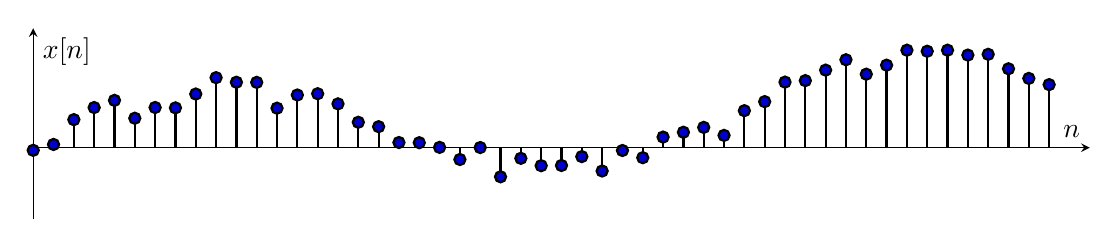
\begin{tikzpicture}
	\begin{axis}[%
		axis x line=middle,
		axis y line=middle,
		ticks=none,
		enlarge x limits=0,
		enlarge y limits=0.15,
		xmin=0,
		xmax=52,
		ymin=-1,
		width=15cm,
		height=4cm,
		domain = 0:50,
		samples = 51,
		xlabel={$n$},
		ylabel={$x[n]$}]
		\addplot+[ycomb,black,thick] {sin(2*180*x/35) + 0.3*rand + x/50};
\end{axis}
\end{tikzpicture}
	\end{center}
\caption{Realizations of a discrete stochastic process}
\label{fig:realizations_stochastic_process}
\end{figure}

\section{Preliminaries: Spectral analysis of deterministic signals}
\label{sec:preliminaries_deterministic_signals}
	
Before going into the spectral analysis of stochastic processes, it is convenient to study the case of deterministic signals, which will help us to understand the concept of spectral resolution. Thus, the problem is to compute the Fourier transform of the deterministic signal $x[n]$. However, this relatively ``simple'' approach has two issues. First, we do not have access to the whole signal $x[n]$, but only to a finite record thereof
\begin{equation}
   x_w[n]  = \begin{cases}
   x[n], & n = 0, \ldots, N-1, \\
   0, & \text{otherwise.}
   \end{cases}
\end{equation}
Defining now the window
\begin{equation}
w_{R,N}[n]  = \begin{cases}
1, & n = 0, \ldots, N-1, \\
0, & \text{otherwise,}
\end{cases}
\end{equation}
we may rewrite $x_w[n] = w_{R,N}[n] x[n]$, which allows us to compute the Fourier transform of $x_w[n]$ as\footnote{In the ``Signals and Systems'' parlance, this Fourier transform is named Discrete Time Fourier Transform (DTFT).}
\begin{equation}
\label{eq:DTFT}
X_w(e^{j \omega}) = \mathcal{F} \left(x_w[n]\right) = \sum_{n = 0}^{N-1} x_w[n] e^{- j \omega N} = \frac{1}{2 \pi} W_{R,N}(e^{j \omega}) \circledast X(e^{j \omega}),
\end{equation}
where $\circledast$ denotes the circular convolution. So, the Fourier transform of the windowed signal, $x_w[n]$, is related to that of $x[n]$ through the Fourier transform of the window $w_{R,N}[n]$, which is given by
\begin{equation}
W_{R,N}(e^{j \omega}) = e^{-j \omega (N-1)/2} \frac{\sin\left(\frac{\omega N}{2}\right)}{\sin\left(\frac{\omega}{2}\right)} = e^{-j \omega (N-1)/2} P_N(e^{j \omega}),
\end{equation}
and its amplitude $|P_N(e^{j \omega})|$ is depicted in Figure \ref{fig:FT_rectangularwindow}. As this figure shows, the width of the main lobe is $4 \pi/N$.

\begin{figure}
	\pgfmathsetmacro{\mypi}{3.141592}
	\pgfmathsetmacro{\windowlength}{10}
	\begin{center}
		\begin{tikzpicture}
		\begin{axis}[%
		axis x line=middle,
		axis y line=middle,
		enlarge x limits=0.05,
		enlarge y limits=0.2,
		xtick={-\mypi,-2*\mypi/\windowlength,2*\mypi/\windowlength,\mypi},
		xticklabels={$-\pi$,$-\frac{2\pi}{N}$,$\frac{2\pi}{N}$,$\pi$},
		xmin=-\mypi,
		xmax=\mypi,
		ymin=0,
		ytick=\empty,
		width=10cm,
		height=7.5cm,
		domain = -\mypi:\mypi,
		samples = 512,
		xlabel={$\omega$},
		ylabel={$|P_N(e^{j \omega})|$}]
		%\addplot+[ycomb,black,thick] {x*\mypi};
		\addplot[black,thick] {abs(sin(deg(x*\windowlength/2))/sin(deg(x/2)))};
		\end{axis}
		\end{tikzpicture}
	\end{center}
	\caption{Module of the Fourier transform of the rectangular window}
	\label{fig:FT_rectangularwindow}
\end{figure}

The second issue is that the DTFT in \eqref{eq:DTFT} is a function of a continuous variable. Hence it cannot be computed nor stored in a computer. The solution is simple and consists in discretizing the spectrum, which yields the Discrete Fourier Transform (DFT). Thus, we are only able to compute $X_w(e^{j \omega_k}),$ with $\omega_k = 2 \pi k/N$ and $k = 0, \ldots, N-1$. The DFT is typically computed using the fast Fourier transform (FFT) algorithm. 

The aforementioned procedure based on the DFT/FFT gets only $N$ samples of the spectrum for length-$N$ signals, but we can get more samples by zero-padding the signals, i.e., by simply adding $N_\text{fft} - N$ zeros after the $N$ samples. This procedure increases the number of frequencies but it does not increase the resolution as it does not modify the window.
	
%%%%%%%%%%%%%%%
\begin{example}[Spectral analysis of a complex exponential]
	\label{ex:spectral_analysis_deterministic}
	
	This example considers the spectral analysis of finite record of a complex exponential, i.e., $x[n] = e^{j \omega_0 n}, n = 0, \ldots, N-1$. Using the DTFT of a complex exponential, given by
\begin{equation}
X(e^{j \omega}) = 2 \pi \delta(\omega - \omega_0),
\end{equation}
and $W_N(e^{j \omega})$, $X_w(e^{j \omega})$ becomes
\begin{equation}
X_w(e^{j \omega}) = e^{-j (\omega - \omega_0) (N-1)/2} \frac{\sin\left(\frac{(\omega - \omega_0) N}{2}\right)}{\sin\left(\frac{\omega - \omega_0}{2}\right)} =  e^{-j (\omega - \omega_0) (N-1)/2} P_N\left(\omega - \omega_0\right),
\end{equation}
and its magnitude squared is
\begin{equation}
|X_w(e^{j \omega})|^2 = \left|P_N\left(e^{j (\omega - \omega_0)}\right)\right|^2.
\end{equation}
Figure \ref{fig:FT_complexexponential} plots, in logarithmic scale, $|X_w(e^{j \omega})|^2$ and $|X_w(e^{j \omega_k})|^2$ for two different values of $N_\text{fft}$.
\begin{figure}
	\pgfmathsetmacro{\mypi}{3.141592}
	\pgfmathsetmacro{\windowlength}{14}
	\pgfmathsetmacro{\myomega}{\mypi/8}
	\begin{center}
		\begin{tikzpicture}
		\begin{axis}[%
		axis x line=bottom,
		axis y line=middle,
		enlarge x limits=0.05,
		enlarge y limits=0.2,
		xtick={-\mypi,\myomega,\mypi},
		xticklabels={$-\pi$,$\omega_0$,$\pi$},
		xmin=-\mypi,
		xmax=\mypi,
		ymin=1e-3,
		ytick=\empty,
		ymode=log,
		width=8cm,
		height=6cm,
		domain = -\mypi:\mypi,
		samples = 512,
		xlabel={$\omega$},
		ylabel={$|X_w(e^{j \omega})|^2$}]
		%\addplot+[ycomb,black,thick] {x*\mypi};
		\addplot[black,thick] {(sin(deg((x-\myomega)*\windowlength/2))/sin(deg((x-\myomega)/2)))^2};
		\addplot+[only marks,mark=*,black,thick,each nth point=32] {(sin(deg((x-\myomega)*\windowlength/2))/sin(deg((x-\myomega)/2)))^2};
		\end{axis}
		\end{tikzpicture}
		\hspace{0.5cm}
		\begin{tikzpicture}
\begin{axis}[%
axis x line=bottom,
axis y line=middle,
enlarge x limits=0.05,
enlarge y limits=0.2,
xtick={-\mypi,\myomega,\mypi},
xticklabels={$-\pi$,$\omega_0$,$\pi$},
xmin=-\mypi,
xmax=\mypi,
ymin=1e-3,
ytick=\empty,
ymode=log,
width=8cm,
height=6cm,
domain = -\mypi:\mypi,
samples = 512,
xlabel={$\omega$},
ylabel={$|X_w(e^{j \omega})|^2$}]
\addplot[black,thick] {(sin(deg((x-\myomega)*\windowlength/2))/sin(deg((x-\myomega)/2)))^2};
\addplot+[only marks,mark=*,black,thick,each nth point=16] {(sin(deg((x-\myomega)*\windowlength/2))/sin(deg((x-\myomega)/2)))^2};
\end{axis}
\end{tikzpicture}
	\end{center}
	\caption{Fourier transform (in logarithmic scale) of a windowed complex exponential}
	\label{fig:FT_complexexponential}
\end{figure}
		
As we have seen in this example, the spectral analysis of deterministic signals depends on two factors. First, the number of available samples, which determines the window and, therefore, the shape of the window spectrum. As we have seen in Figure \ref{fig:FT_complexexponential}, the rectangular window has a narrow main lobe at the expense of high secondary lobes. This effect could be reduced by pre-multiplying $x_w[n]$ by a different window, which would reduce the height of the secondary lobes, but it would widen the main lobe.

\end{example}
%%%%%%%%%%%%%

%%%%%%%%%%%%%%%
\begin{example}[Spectral analysis of two complex exponentials]
	\label{ex:spectral_analysis_deterministic_two}
	
	This example considers the spectral analysis of finite record of the sum of two complex exponential, i.e., $x[n] = e^{j \omega_0 n} + e^{j \omega_1 n}, n = 0, \ldots, N-1$, which will help us to understand the concept of resolution. Using \eqref{eq:DTFT}, we have
	\begin{equation}
	X_w(e^{j \omega}) = e^{-j (\omega - \omega_0) (N-1)/2} P_N\left(\omega - \omega_0\right)+  e^{-j (\omega - \omega_1) (N-1)/2} P_N\left(\omega - \omega_1\right).
	\end{equation}
	and its magnitude squared is
	\begin{multline}
	|X_w(e^{j \omega})|^2 = \left|P_N\left(e^{j (\omega - \omega_0)}\right)\right|^2 + \left|P_N\left(e^{j (\omega - \omega_1)}\right)\right|^2  \\  + e^{j (\omega_0 - \omega_1) (N-1)/2} P_N\left(e^{j (\omega - \omega_0)}\right) P_N\left(e^{j (\omega - \omega_1)}\right)\\ +  e^{- j (\omega_0 - \omega_1) (N-1)/2} P_N\left(e^{j (\omega - \omega_0)}\right) P_N\left(e^{j (\omega - \omega_1)}\right).
\end{multline}
Taking into account Euler's formula, $|X_w(e^{j \omega})|^2$ can be simplified as
	\begin{multline}
|X_w(e^{j \omega})|^2 = \left|P_N\left(e^{j (\omega - \omega_0)}\right)\right|^2 + \left|P_N\left(e^{j (\omega - \omega_1)}\right)\right|^2  \\  + 2 \cos \left(\frac{(\omega_0 - \omega_1) (N-1)}{2} \right) P_N\left(e^{j (\omega - \omega_0)}\right) P_N\left(e^{j (\omega - \omega_1)}\right).
\end{multline}
Figure \ref{fig:FT_twocomplexexponential} plots, in logarithmic scale, $|X_w(e^{j \omega})|^2$ for two different separations between the frequencies of the exponentials. As we can see in this figure, for small frequency separations, it is impossible to identify in the spectrum the two complex exponentials.
	\begin{figure}
		\pgfmathsetmacro{\mypi}{3.141592}
		\pgfmathsetmacro{\windowlength}{14}
		\pgfmathsetmacro{\myomega}{\mypi/8}
		\pgfmathsetmacro{\myomegabis}{3*\mypi/8}
		\pgfmathsetmacro{\myomegabisbis}{1.5*\mypi/8}
		\begin{center}
	\begin{tikzpicture}
\begin{axis}[%
axis x line=bottom,
axis y line=middle,
enlarge x limits=0.05,
enlarge y limits=0.2,
xtick={-\mypi,\myomega,\myomegabis,\mypi},
xticklabels={$-\pi$,$\omega_0$,$\omega_1$,$\pi$},
xmin=-\mypi,
xmax=\mypi,
ymin=1e-3,
ytick=\empty,
ymode=log,
width=8cm,
height=6cm,
domain = -\mypi:\mypi,
samples = 512,
xlabel={$\omega$},
ylabel={$|X_w(e^{j \omega})|^2$}]
\addplot[black,thick] {(sin(deg((x-\myomega)*\windowlength/2))/sin(deg((x-\myomega)/2)))^2 + (sin(deg((x-\myomegabis)*\windowlength/2))/sin(deg((x-\myomegabis)/2)))^2  + 2*cos(deg((\myomega - \myomegabis)*(\windowlength - 1)/2))*(sin(deg((x-\myomega)*\windowlength/2))/sin(deg((x-\myomega)/2)))*(sin(deg((x-\myomegabis)*\windowlength/2))/sin(deg((x-\myomegabis)/2)))};
\end{axis}
\end{tikzpicture}
	\begin{tikzpicture}
\begin{axis}[%
axis x line=bottom,
axis y line=middle,
enlarge x limits=0.05,
enlarge y limits=0.2,
xtick={-\mypi,\myomega,\mypi},
xticklabels={$-\pi$,$\omega_0$,$\pi$},
extra x ticks={\myomegabisbis},
extra x tick labels={$\omega_1$},
extra x tick style={tick label style={yshift=5mm}},
xmin=-\mypi,
xmax=\mypi,
ymin=1e-3,
ytick=\empty,
ymode=log,
width=8cm,
height=6cm,
domain = -\mypi:\mypi,
samples = 512,
xlabel={$\omega$},
ylabel={$|X_w(e^{j \omega})|^2$}]
\addplot[black,thick] {(sin(deg((x-\myomega)*\windowlength/2))/sin(deg((x-\myomega)/2)))^2 + (sin(deg((x-\myomegabisbis)*\windowlength/2))/sin(deg((x-\myomegabisbis)/2)))^2  + 2*cos(deg((\myomega - \myomegabisbis)*(\windowlength - 1)/2))*(sin(deg((x-\myomega)*\windowlength/2))/sin(deg((x-\myomega)/2)))*(sin(deg((x-\myomegabisbis)*\windowlength/2))/sin(deg((x-\myomegabisbis)/2)))};
\end{axis}
\end{tikzpicture}
		\end{center}
		\caption{Fourier transform (in logarithmic scale) of the sum of two complex exponentials}
		\label{fig:FT_twocomplexexponential}
	\end{figure}
	
\end{example}
%%%%%%%%%%%%%

\section{Non-parametric methods in spectral estimation}

In this section, we turn our attention to the case of stochastic signals and, in particular, to the development of non-parametric spectral estimation methods. We will therefore study the periodogram and variations thereof. 

Before proceeding, let us note that throughout this section, we will only consider DTFTs. However, we have to keep in mind that, in practice, we can only compute the DFT (using the FFT algorithm), as we have seen in Section \ref{sec:preliminaries_deterministic_signals}.

\subsection{The periodogram}

Despite the title section, we will start with a estimator known as correlogram, which is based on a first definition of the PSD.
\begin{definition}
	\label{wiener_khinchin}
	Given a WSS process $x[n]$, the power spectral density is defined as
	\begin{equation}
	S_x(e^{j \omega}) = \mathcal{F}(r_{x}[m]),
	\end{equation}
	where
	\begin{equation}
	r_{x}[m] = \mathbb{E}[x[n] x^{\ast}[n-m]],
	\end{equation}
	is the auto-correlation function of the process $x[n]$.
\end{definition}

Based on Definition \ref{wiener_khinchin}, the first estimator of the PSD is given by
\begin{equation}
	\hat{S}_x(e^{j \omega}) = \mathcal{F}(\hat{r}_{x}[m]),
\end{equation}
where $\hat{r}_{x}[m]$ is an estimator of the auto-correlation function. Concretely, we have two alternatives for this estimator: a biased and an unbiased estimator. The biased estimator of the auto-correlation, given the finite length $x[n], n = 0, \ldots, N-1$, is
\begin{equation}
	\label{eq:autocorrelation_biased}
	\hat{r}_{x}^{b}[m] = \frac{1}{N} \sum_{n = m}^{N-1} x[n] x^{\ast}[n-m], \quad m = 0, \ldots, N-1,
\end{equation}
and $\hat{r}_{x}^{b}[m] = \left[ \hat{r}_{x}^{b}[-m] \right]^{\ast}, m = -N+1, \ldots, -1$, whereas the unbiased estimator is
\begin{equation}
	\label{eq:autocorrelation_unbiased}
\hat{r}_{x}^{u}[m] = \frac{1}{N-m} \sum_{n = m}^{N-1} x[n] x^{\ast}[n-m], \quad m = 0, \ldots, N-1,
\end{equation}
and $\hat{r}_{x}^{u}[m] = \left[ \hat{r}_{x}^{u}[-m] \right]^{\ast}, m = -N+1, \ldots, -1$. Consequently, the PSD estimators are
\begin{equation}
\label{eq:correlogram}
\hat{S}_x^{b}(e^{j \omega}) = \mathcal{F}(\hat{r}_{x}^{b}[m]),
\end{equation}
and
\begin{equation}
\hat{S}_x^{u}(e^{j \omega}) = \mathcal{F}(\hat{r}_{x}^{u}[m]).
\end{equation}
Actually, only the estimator in \eqref{eq:correlogram}, which is known as the correlogram, is a valid PSD estimator since it ensures $\hat{S}_x^{b}(e^{j \omega}) \geq 0$, whereas $\hat{S}_x^{u}(e^{j \omega}) \not \geq 0$.

The periodogram, which is a term coined by Arthur Schuster in 1898, is based on a second definition of the power spectral density. This definition states that
\begin{equation}
	S_x(e^{j \omega}) = \lim_{N \rightarrow \infty} \ E \left[\frac{1}{2N -1} \left| \sum_{n = -N+1}^{N-1} x[n] e^{-j \omega n} \right|^2 \right].
\end{equation}
The periodogram is obtained from the above definition by simply dropping the expectation and considering a finite number of samples, i.e.,
\begin{equation}
	\label{eq:periodogram}
	\hat{S}_x^{p}(e^{j \omega}) = \frac{1}{N} \left| \sum_{n = 0}^{N-1} x[n] e^{-j \omega n} \right|^2 = \frac{1}{N} \left| X(e^{j \omega}) \right|^2,
\end{equation}
where $X(e^{j \omega})  = \mathcal{F}(x[n])$.

In the following, we will shed some light on why we have started this section with the correlogram. Let us start by rewriting $\hat{r}_{x}^{b}[m]$ as
\begin{equation}
\hat{r}_{x}^{b}[m] = \frac{1}{N} \sum_{n = m}^{N-1} x[n] x^{\ast}[n-m] = \frac{1}{N} \sum_{n = -\infty}^{\infty} x[n] x^{\ast}[n-m]  = \frac{1}{N} \left(x[n] \ast x^{\ast}[-n]\right),
\end{equation}
and taking its Fourier transform yields
\begin{equation}
\hat{S}_x^{b}(e^{j \omega}) = \mathcal{F}(\hat{r}_{x}^{b}[m]) = \frac{1}{N} \mathcal{F} \left(x[n] \ast x^{\ast}[-n]\right).
\end{equation}
Finally, applying the properties of the Fourier transform, $\hat{S}_x^{b}(e^{j \omega})$ simplifies to
\begin{equation}
\hat{S}_x^{b}(e^{j \omega}) = \frac{1}{N} \mathcal{F} \left(x[n] \right) \mathcal{F} \left(x^{\ast}[-n]\right) = \frac{1}{N} X(e^{j \omega}) X^{\ast}(e^{j \omega}) = \frac{1}{N} \left| X(e^{j \omega}) \right|^2 = \hat{S}_x^{p}(e^{j \omega}),
\end{equation}
which is the periodogram in \eqref{eq:periodogram}. That is, the periodogram and the correlogram are identical.

\subsubsection{Bias and variance of the periodogram}

To understand why we need more refined estimators of the power spectral density, now we shall perform the statistical analysis of the periodogram (or correlogram), i.e.,  we will compute its bias and variance.

The first question is whether the periodogram is a biased estimator of the PSD, that is, 
\begin{equation}
E\left[\hat{S}_x^{p}(e^{j \omega}) \right] \mathop{=}^{?} S_x(e^{j \omega}).
\end{equation}
To compute the bias of the periodogram, it is easier to consider the equivalence with the correlogram, which allows us to write
\begin{equation}
E\left[\hat{S}_x^{p}(e^{j \omega}) \right] = E\left[\mathcal{F}(\hat{r}_{x}^{b}[m]) \right] = \mathcal{F}\left(E\left[ \hat{r}_{x}^{b}[m]\right]\right),  
\end{equation}
where we have used that the expectation and the Fourier transform are both linear operators. Thus, the periodogram is biased if $\hat{r}_{x}^{b}[m]$ is a biased estimate of the auto-correlation function. Now, using the definition of  $\hat{r}_{x}^{b}[m]$, we get\footnote{It is easy to prove that $\hat{r}_{x}^{u}[m]$ is indeed an unbiased estimate of the auto-correlation function, which is left as an exercise for the reader.}
\begin{multline}
E\left[ \hat{r}_{x}^{b}[m]\right] = E\left[ \frac{1}{N} \sum_{n = m}^{N-1} x[n] x^{\ast}[n-m] \right] = \frac{1}{N} \sum_{n = m}^{N-1} E\left[ x[n] x^{\ast}[n-m] \right] \\ = \frac{1}{N} \sum_{n = m}^{N-1} r_{x}[m] = \frac{N - |m|}{N} r_{x}[m] \neq r_{x}[m],
\end{multline}
which shows that $\hat{r}_{x}^{b}[m]$ is indeed a biased estimate of the auto-correlation function, with the exception of $m = 0$, and makes the periodogram a biased estimate of the PSD.

It is possible to obtain a closed-form expression for the bias of the periodogram by noting that
\begin{equation}
\label{eq:bias_auto-correlation}
E\left[\hat{r}_{x}^{b}[m]\right]  = \frac{N - |m|}{N} r_{x}[m] = w_{T,N}[m] r_{x}[m],
\end{equation}
where the triangular, or Barlett window, is defined as
\begin{equation}
w_{T,N}[m] = \begin{cases} \frac{N - |m|}{N}, & |m| \leq N-1, \\
0, & \text{otherwise},
\end{cases}
\end{equation}
and is depicted in Figure \ref{fig:triangularwindow}. The bias given in \eqref{eq:bias_auto-correlation} shows us that the larger the $m$ the larger the bias.
\begin{figure}
	\pgfmathsetmacro{\windowlength}{10}
	\begin{center}
		\begin{tikzpicture}
		\begin{axis}[%
		axis x line=middle,
		axis y line=middle,
		ticks=none,
		enlarge x limits=0.1,
		enlarge y limits=0.15,
		xmin=-\windowlength,
		xmax=\windowlength,
		ymin=0,
		ymax=1.2,
		width=10cm,
		height=7.5cm,
		domain = -\windowlength:\windowlength,
		samples = 2*\windowlength + 1,
		xlabel={$m$},
		ylabel={$w_{T,N}[m]$}]
		\addplot+[ycomb,black,thick] {(\windowlength - abs(x))/\windowlength};
		\end{axis}
		\end{tikzpicture}
	\end{center}
	\caption{Triangular window}
	\label{fig:triangularwindow}
\end{figure}


Using \eqref{eq:bias_auto-correlation}, the bias of the periodogram becomes
\begin{equation}
\label{eq:bias_periodogram}
E\left[\hat{S}_x^{p}(e^{j \omega}) \right] = \mathcal{F}\left(w_{T,N}[m] r_{x}[m]\right) = \frac{1}{2 \pi} W_{T,N}(e^{j \omega}) \circledast S_x(e^{j \omega}),
\end{equation}
where
\begin{equation}
W_{T,N}(e^{j \omega}) = \mathcal{F}\left(w_{T,N}[m]\right) = \frac{1}{N} \mathcal{F}\left(w_{R,N}[m] \ast w_{R,N}[-m]\right) = |W_{R,N}(e^{j \omega})|^2 = \frac{1}{N} \frac{\sin^2\left(\frac{\omega N}{2}\right)}{\sin^2\left(\frac{\omega}{2}\right)}
\end{equation}
is the Fourier transform of the triangular window and is depicted in Figure \ref{fig:FT_triangularwindow}. Comparing Figures \ref{fig:FT_rectangularwindow} and \ref{fig:FT_triangularwindow}, it can be seen that the level of secondary lobes is smaller for the triangular window. By analogy with Example \ref{ex:spectral_analysis_deterministic_two}, we can say that the bias of the periodogram is related with its resolution.

\begin{figure}
	\pgfmathsetmacro{\mypi}{3.141592}
	\pgfmathsetmacro{\windowlength}{10}
	\begin{center}
		\begin{tikzpicture}
		\begin{axis}[%
		axis x line=middle,
		axis y line=middle,
		enlarge x limits=0.05,
		enlarge y limits=0.2,
		xtick={-\mypi,-2*\mypi/\windowlength,2*\mypi/\windowlength,\mypi},
		xticklabels={$-\pi$,$-\frac{2\pi}{N}$,$\frac{2\pi}{N}$,$\pi$},
		xmin=-\mypi,
		xmax=\mypi,
		ymin=0,
		ytick=\empty,
		width=10cm,
		height=7.5cm,
		domain = -\mypi:\mypi,
		samples = 512,
		xlabel={$\omega$},
		ylabel={$W_{T,N}(e^{j \omega})$}]
		\addplot[black,thick] {(sin(deg(x*\windowlength/2))/sin(deg(x/2)))^2};
		\end{axis}
		\end{tikzpicture}
	\end{center}
	\caption{Fourier transform of the triangular window}
	\label{fig:FT_triangularwindow}
\end{figure}

We have shown in \eqref{eq:bias_periodogram} that the periodogram is biased. However, there are some cases when it is not. For instance, considering the asymptotic regime, it is unbiased:
\begin{equation}
\lim_{N \rightarrow \infty} \hat{S}_x^{p}(e^{j \omega}) = S_x(e^{j \omega}).
\end{equation}
Another case is when the process $x[n]$ is white noise. For this kind of processes, $r_{x}[m] = \sigma^2_x \delta[m]$ and, therefore
\begin{equation}
E\left[\hat{r}_{x}^{b}[m]\right]  = \frac{N - |m|}{N} r_{x}[m] = \sigma^2_x \delta[m] = r_{x}[m].
\end{equation}
Since the estimate of the auto-correlation is unbiased for white processes, it is easy to show that the periodogram is also unbiased.

The analysis of the variance of the periodogram is cumbersome and can only be done in particular cases. For white noise, it can be shown that
\begin{equation}
 \mathop{Var}\left(\hat{S}_x^{p}(e^{j \omega})\right) = S_x^{2}(e^{j \omega}),
\end{equation}
and in general we can say that
\begin{equation}
\mathop{Var}\left(\hat{S}_x^{p}(e^{j \omega})\right) \appropto S_x^{2}(e^{j \omega}),
\end{equation}
where $\appropto$ denotes approximately proportional to.  This expression tells us that the variance does not decrease for larger data records. That is, the periodogram is not a consistent estimate of the PSD.

\subsection{The Blackman-Tukey estimator}

One of the reasons for the behavior of the periodogram variance is the poor quality of the estimate $\hat{r}_{x}^{b}[m]$ for values of $m$ close to $N$. This problem is what the Blackman-Tukey (BT) estimator tries to improve. The idea is to ignore or weight the samples of $\hat{r}_{x}^{b}[m]$ for $m$ close to $N$. Thus, the BT estimator is
\begin{equation}
\label{eq:BT_definition}
\hat{S}_x^{BT}(e^{j \omega}) = \mathcal{F}(w_M[m] \hat{r}_{x}^{b}[m]) = \sum_{m = -N + 1}^{N-1} w_M[m] \hat{r}_{x}^{b}[m] e^{-j \omega m},
\end{equation}
where $w[m]$ is a window that must fulfill
\begin{equation}
w_{M}[m] = \begin{cases} f(|m|), & |m| \leq M-1, \\
0, & \text{otherwise},
\end{cases}
\end{equation}
where $f(|m|)$ is a monotonically decreasing function of $|m|$ and $M \leq N$. This window ignores the lags of the estimated auto-correlation for $|m|>M-1$ and weights  the lags for large $m$. The choice of the window  is critical to achieve good performance, but, in any case, it must guarantee that $\hat{S}_x^{p}(e^{j \omega}) \geq 0$.

Using the properties of the Fourier transform, we may rewrite $\hat{S}_x^{p}(e^{j \omega})$ as
\begin{equation}
\label{eq:BT_convolution}
\hat{S}_x^{BT}(e^{j \omega}) = \frac{1}{2 \pi} W_M(e^{j \omega}) \circledast \hat{S}_x^{p}(e^{j \omega}) = \frac{1}{2 \pi} \int_{-\pi}^{\pi} \hat{S}_x^{p}(e^{j \psi}) W_{M}(e^{j (\omega - \psi)}) d \psi,
\end{equation} 
where $W_M(e^{j \omega}) = \mathcal{F}(w_M[n])$. Then, the Blackman-Tukey estimator is locally smoothing the periodogram, which reduces its variance. However, there is no free lunch and we will show that this variance reduction translates into lower resolution (or larger bias). Concretely, the bias of the BT estimator is
\begin{equation}
\label{eq:BT_convolution}
E\left[\hat{S}_x^{BT}(e^{j \omega})\right] = \frac{1}{2 \pi} W_M(e^{j \omega}) \circledast E\left[\hat{S}_x^{p}(e^{j \omega})\right] = \frac{1}{2 \pi} W_M(e^{j \omega}) \circledast  W_{T,N}(e^{j \omega}) \circledast S_x(e^{j \omega}).
\end{equation}
Finally, since $w_M[n]$ is shorter than $w_{T,N}[n]$, it can be shown that $W_M(e^{j \omega})$ is wider than $W_{T,M}(e^{j \omega})$, which translates into a lower resolution. This behavior is depicted in Figure \ref{fig:comparison_windows} for $w_M[n] = w_{T,M}[n]$. Note that the $y$-axis is in logarithmic scale.
\begin{figure}
	\pgfmathsetmacro{\mypi}{3.141592}
	\pgfmathsetmacro{\windowlength}{10}
	\pgfmathsetmacro{\windowlengthbis}{6}
	\begin{center}
		\begin{tikzpicture}
		\begin{axis}[%
		axis x line=bottom,
		axis y line=middle,
		enlarge x limits=0.05,
		enlarge y limits=0.2,
		xtick={-\mypi,-2*\mypi/\windowlengthbis,-2*\mypi/\windowlength,2*\mypi/\windowlength, 2*\mypi/\windowlengthbis,\mypi},
		xticklabels={$-\pi$,$-\frac{2\pi}{M}$,$-\frac{2\pi}{N}$,$\frac{2\pi}{N}$,$\frac{2\pi}{M}$,$\pi$},
		xmin=-\mypi,
		xmax=\mypi,
		ymin=1e-3,
		ymode=log,
		ytick=\empty,
		width=10cm,
		height=7.5cm,
		domain = -\mypi:\mypi,
		samples = 512,
		xlabel={$\omega$}]
		\addplot[black,thick] {(sin(deg(x*\windowlength/2))/sin(deg(x/2)))^2};
		\addplot[blue,thick] {2.8*(sin(deg(x*\windowlengthbis/2))/sin(deg(x/2)))^2};
		\legend{$W_{T,N}(e^{j \omega})$,$W_{T,M}(e^{j \omega})$};
		\end{axis}
		\end{tikzpicture}
	\end{center}
	\caption{Fourier transform (in logarithmic scale) of two triangular windows of different lengths}
	\label{fig:comparison_windows}
\end{figure}

\subsection{Estimators based on the averaged periodogram}

The Blackman-Tukey estimator yields a smaller variance than that of the periodogram because, as we have seen, it smooths the periodogram. An alternative to reduce the variance is to average several periodograms. However, the question is: How do we obtain such periodograms? The answer is easy and consists in dividing the $N$ observations into windows of length $M < N$. 

The Barlett method is one of the possible estimators based on the averaged periodogram. First, it divides the $N$ observations into $L$ non-overlapping windows of length $M$ as
\begin{equation}
	x_l[n] = x[(l-1) M + n],
\end{equation}
where $n = 0, \ldots, M-1$ and $l = 1, \ldots, L$, and computes the periodogram of each window, that is,
\begin{equation}
\hat{S}_{x,l}^{p}(e^{j \omega}) = \frac{1}{M} \left| \sum_{n = 0}^{M-1} x_l[n] e^{-j \omega n} \right|^2 = \frac{1}{M} \left| X_l(e^{j \omega}) \right|^2.
\end{equation}
Then, the estimator is given by simply averaging the individual periodograms
\begin{equation}
\label{eq:Barlett_estimator}
\hat{S}_{x}^{B}(e^{j \omega}) = \frac{1}{L} \sum_{l = 1}^{L}\hat{S}_{x,l}^{p}(e^{j \omega}).
\end{equation}
Although it is out of the scope of these notes, we must point out that $\hat{S}_{x}^{B}(e^{j \omega})$ is somehow related to $\hat{S}_{x}^{BT}(e^{j \omega})$.

There are two further improvements of the periodogram. The first one is based on the Barlett estimator but substituting the individual periodograms by Blackman-Tukey estimates. The second one is based on dividing the $N$ observations into $L$ overlapping windows. The combination of both improvements is known as the Welch method.

One final question remains: What happens to the bias and variance of these methods. Regarding the bias (resolution), it is going to be smaller than that of the periodogram since $M < N$, as also happened to the Blackman-Tukey estimate. As for the variance, it is going to be reduced by a factor of $L$, the number of windows. That is,
\begin{equation}
\mathop{Var}\left(\hat{S}_x^{ap}(e^{j \omega})\right) \approx \frac{1}{L} \mathop{Var}\left(\hat{S}_x^{p}(e^{j \omega})\right),
\end{equation}
where $\hat{S}_x^{ap}(e^{j \omega})$ is any averaged periodogram (either Barlett or Welch methods) and $\approx$ is due to the non-independence between the windows. It would be an equality when the windows are independent, i.e., the Barlett method.

\section{Parametric methods in spectral estimation}

The problem of non-parametric methods is that they estimate an infinite number of parameters (the PSD at each frequency) from a sequence of $N$ observations. Clearly, this is an ill-posed problem since there are (many) more parameters to estimate than observations. To overcome this issue, we could postulate a parametric model for the PSD and estimate only the parameters of such model using the $N$ observations. For instance, the model could be $S_x(e^{j \omega})  = a + b \cos^2(\omega)$ and, hence, we only have to estimate $a$ and $b$.

Parametric approaches, as described above, can provide a significant performance boost if the signal fits the postulated model, otherwise the performance could be even worse than that of non-parametric methods. It is therefore of the utmost importance to select the proper model.

\subsection{Rational models for parametric spectral estimation}

These models consider a white Gaussian noise $u[n]$ with zero mean and variance $\sigma^2$ that goes through a causal and stable filter\footnote{A filter is said to be causal and stable if and only if all its poles are inside the unit circle.} $h[n]$ that has the following Fourier transform
\begin{equation}
	H(e^{j \omega}) = \frac{B(e^{j \omega})}{A(e^{j \omega})} = \frac{\displaystyle \sum_{k = 0}^{q} b_k e^{-j \omega k}}{\displaystyle 1 + \sum_{k = 1}^{p} a_k e^{-j \omega k}},
\end{equation}
which implies that
\begin{equation}
	\label{eq:signal_model_ARMA}
	x[n] = u[n] \ast h[n] = - \sum_{k = 1}^{p} a_k x[n -k] + \sum_{k = 0}^{q} b_k u[n-k].
\end{equation}
For these models, the PSD  is given by
\begin{equation}
\label{eq:PSD_ARMA}
S_x(e^{j \omega}) = S_u(e^{j \omega}) |H(e^{j \omega})|^2 = \sigma^2 \left|\frac{\displaystyle \sum_{k = 0}^{q} b_k e^{-j \omega k}}{\displaystyle 1 + \sum_{k = 1}^{p} a_k e^{-j \omega k}}\right|^2,
\end{equation}
and we only have to estimate $\sigma^2$, $a_1, \ldots, a_p$, and $b_0, \ldots, b_q$. 

According to Weierstrass theorem, for large values $p$ and $q$, the PSD model in \eqref{eq:PSD_ARMA} can approximate arbitrarily close any continuous PSD. Hence, there is a strong interest in this kind of models, which are named as auto-regressive moving average (ARMA or ARMA(p,q)). There are two special cases of the ARMA model that are particularly interesting: the auto-regressive (AR or AR(p)) and the moving average (MA or MA(q)). For the former, the PSD is given by
\begin{equation}
\label{eq:PSD_AR}
S_x(e^{j \omega}) = \frac{\sigma^2}{\displaystyle \left|1 + \sum_{k = 1}^{p} a_k e^{-j \omega k}\right|^2},
\end{equation}
whereas, for the latter, it is
\begin{equation}
\label{eq:PSD_ARMA}
S_x(e^{j \omega}) =  \sigma^2 \left|\sum_{k = 0}^{q} b_k e^{-j \omega k}\right|^2.
\end{equation}
AR models are good choices if we suspect the PSD has large peaks and MA models are good choices for PSDs with large valleys.

The estimation of the model parameters is typically carried out in the time domain, for which the auto-correlation structure is required. Once the auto-correlation function is available, which will depend in general on the model parameters in a non-linear fashion, the estimation procedure consists in substituting the theoretical auto-correlation by an estimate and then solving a non-linear system of equations. The PSD estimate is obtained by substituting the estimated parameters in the corresponding model. This procedure, which is conceptually simple, is actually rather involved. However, there is an exception, which is the AR model since the dependency of auto-correlation on the parameters is linear.

\subsection{The auto-correlation function of ARMA processes}

This section computes the auto-correlation function of ARMA processes, which is defined as
\begin{equation}
	r_{x}[m] = \mathbb{E}[x[n] x^{\ast}[n-m]].
\end{equation}
Substituting $x[n]$ by \eqref{eq:signal_model_ARMA}, $r_{x}[m]$ becomes
\begin{align}
r_{x}[m] &= E\left[ \left(- \sum_{k = 1}^{p} a_k x[n -k]  + \sum_{k = 0}^{q} b_k u[n-k] \right) x^{\ast}[n-m]\right] \nonumber \\
&=  - \sum_{k = 1}^{p} a_k E\left[x[n -k] x^{\ast}[n-m]\right] + \sum_{k = 0}^{q} b_k  E\left[u[n-k]  x^{\ast}[n-m]\right] \nonumber \\
&=  - \sum_{k = 1}^{p} a_k r_{x}[m-k] + \sum_{k = 0}^{q} b_k  r_{ux}[m-k].
\end{align}
where the cross-correlation function between $u[n]$ and $x[n]$ is
\begin{equation}
r_{ux}[m] =   E\left[u[n]  x^{\ast}[n-m]\right].
\end{equation}
Now, taking into account that
\begin{equation}
x[n] = u[n] \ast h[n] = \sum_{l = -\infty}^{\infty} h[l] u[n-l],
\end{equation}
the cross-correlation function becomes
\begin{align}
r_{ux}[m] &=   E\left[u[n]  \sum_{l = -\infty}^{\infty} h^{\ast}[l] u^{\ast}[n-m-l]\right] \nonumber \\
&=   \sum_{l = -\infty}^{\infty} h^{\ast}[l] E\left[u[n]   u^{\ast}[n-m-l]\right] \nonumber \\
&=   \sum_{l = -\infty}^{\infty} h^{\ast}[l] r_u [m+l], \nonumber \\
&=   \sum_{l = -\infty}^{\infty} h^{\ast}[-l] r_u [m-l], \nonumber \\
&=   r_u [m] \ast h^{\ast}[-m],
\end{align}
where the auto-correlation of $u[n]$ is
\begin{equation}
r_{u}[m] = \mathbb{E}[u[n] u^{\ast}[n-m]] = \sigma^2 \delta[m],
\end{equation}
because it is a white process. Then, $r_{ux}[m]$ simplifies to
\begin{equation}
r_{ux}[m] =  \sigma^2 h^{\ast}[-m],
\end{equation}
and plugging $r_{ux}[m]$ into $r_{x}[m]$, the desired auto-correlation becomes
\begin{equation}
r_{x}[m] =  - \sum_{k = 1}^{p} a_k r_{x}[m-k] + \sigma^2 \sum_{k = 0}^{q} b_k  h^{\ast}[k-m].
\end{equation}
The second term in the right-hand side of the the above equation can be expanded as
\begin{equation}
\sigma^2 \sum_{k = 0}^{q} b_k  h^{\ast}[k-m] = \sigma^2  \left(b_0 h[-m] + b_1 h[1-m] + \ldots + b_q h[q-m]\right),
\end{equation}
and since the filter is causal ($h[m] = 0, \forall m<0$), it becomes
\begin{align}
\sigma^2  \sum_{k = 0}^{q} b_k  h^{\ast}[k-m] &= \begin{cases}
\sigma^2  \left(b_m h[0] + b_{m+1} h[1] + \ldots + b_q h[q-m]\right), & 0 \leq  m \leq q, \\ 
0, & m > q,
\end{cases} \nonumber \\
&= \begin{cases}
\displaystyle \sigma^2  \sum_{k = m}^{q} b_k  h^{\ast}[k-m], & 0 \leq  m \leq q, \\ 
0, & m > q.
\end{cases}
\end{align}
Putting all pieces together we get
\begin{equation}
\label{eq:correlation_ARMA}
r_{x}[m] = \begin{cases}
\displaystyle - \sum_{k = 1}^{p} a_k r_{x}[m-k] + \sigma^2  \sum_{k = m}^{q} b_k  h^{\ast}[k-m], & 0 \leq  m \leq q, \\ 
\displaystyle  - \sum_{k = 1}^{p} a_k r_{x}[m-k], & m > q, \\
r_{x}^{\ast}[-m], & m < 0.
\end{cases}
\end{equation}
Keeping in mind that $h[m]$ will depend on $a_1, \ldots, a_p$, and $b_0, \ldots, b_q$, it is easy to see in \eqref{eq:correlation_ARMA} that the relationship between the model parameters ($\sigma^2$, $a_1, \ldots, a_p$, and $b_0, \ldots, b_q$) and the auto-correlation is non-linear, which complicates tremendously the estimation of such parameters from an estimate of the auto-correlation function. This is shown in the following example for a particular ARMA model.

\begin{example}[Auto-correlation function of an ARMA(1,1) process]
	
In this example, we will consider an ARMA(1,1) process, which has the following frequency response
\begin{equation}
H(e^{j \omega}) = \frac{1 - b e^{-j \omega}}{1 - a e^{-j \omega}},
\end{equation}
and the corresponding impulse response is
\begin{equation}
h[n] = a^n u[n] - b a^{n-1} u[n-1],
\end{equation}
where
\begin{equation}
u[n] = \begin{cases}
1, & n \geq 0, \\
0, & n < 0.
\end{cases}
\end{equation}
Now, we specialize \eqref{eq:correlation_ARMA} for the case of $p = 1, q = 1, b_0 = 1, b_1 = -b,$ and $a_1 = -a$, which yields
\begin{align*}
	r_x[0] &= a r_x[-1]  + \sigma^2 \left(1 + (-b) (a-b)^{\ast}\right), \\
	r_x[1] &= a r_x[0]  + \sigma^2  (-b), \\
	r_x[2] &= a r_x[1] , \\
	r_x[3] &= a r_x[2] , \\
	&\phantom{=} \vdots
\end{align*}
where we have taken into account that $h[0] = 1$ and $h[1] = a - b$. To recover the three model parameters, we need three equations, which are
\begin{equation}
	\begin{bmatrix}
	r_x[0] & r_x[-1] \\
	r_x[1] & r_x[0] \\
	r_x[2] & r_x[1] 
	\end{bmatrix}
	\begin{bmatrix}
	1 \\ -a
	\end{bmatrix} = 
	\begin{bmatrix}
	\sigma^2 \left(1 - b (a-b)^{\ast}\right) \\
	\sigma^2  (-b) \\
	0
	\end{bmatrix}.
\end{equation}
The first issue to solve the above system of equations is that we do not know $r_x[m]$, but as explained before it can be substituted by any estimator of the auto-correlation function, such as \eqref{eq:autocorrelation_biased} or \eqref{eq:autocorrelation_unbiased}, yielding
\begin{equation}
	\begin{bmatrix}
	\hat{r}_x[0] & \hat{r}_x^{\ast}[1] \\
	\hat{r}_x[1] & \hat{r}_x[0] \\
	\hat{r}_x[2] & \hat{r}_x[1] 
\end{bmatrix}
\begin{bmatrix}
	1 \\ -a
\end{bmatrix} = 
\begin{bmatrix}
	\sigma^2 \left(1 - b (a-b)^{\ast}\right) \\
	\sigma^2  (-b) \\
	0
\end{bmatrix},
\end{equation}
where we have used $\hat{r}_x[-1] = \hat{r}_x^{\ast}[1]$. The second issue is that the system of equations is non-linear, which makes it difficult to solve, even for this simple ARMA model.
\end{example}

\subsection{AR processes}

In the following, we will consider AR (= ARMA(p,0)) processes, which are the most commonly used ones among the three kind of processes studied in this course. There are several reasons. The first one is that the estimation of the parameters is much simpler. Actually, it can be done by simply solving a system of equations. Moreover, from the expression of an AR model
\begin{equation}
\label{eq:signal_model_AR}
x[n]  = u[n] - \sum_{k = 1}^{p} a_k x[n -k],
\end{equation}
where we have assumed without loss of generality that $b_0 = 1$, we note that they can be used to predict future samples by ignoring the input, i.e.,
\begin{equation}
\label{eq:linear_prediction}
x[n]  =  - \sum_{k = 1}^{p} \hat{a}_k x[n -k],
\end{equation}
where the coefficient of the model have been replaced by some estimates. That is, from a record of $N$ samples, $x[0], \ldots, x[N-1]$, we can estimate the model parameters and, afterwards, we can predict $x[N], x[N+1], \ldots$

Let's now turn our attention to the estimation of the AR model parameters. Before proceeding, we shall require the impulse response of the system, which is given by
\begin{equation}
h[n] = \left.x[n]\right|_{u[n] = \delta[n]} = \delta[n] - \sum_{k = 1}^{p} a_k h[n -k],
\end{equation}
and since the filter is causal, we find that $h[0] = 1$, and allows us to particularize \eqref{eq:correlation_ARMA} as follows
\begin{equation}
\label{eq:correlation_AR}
r_{x}[m] = \begin{cases}
\displaystyle - \sum_{k = 1}^{p} a_k r_{x}[m-k] + \sigma^2  \overbrace{h^{\ast}[0]}^1, & m = 0, \\ 
\displaystyle  - \sum_{k = 1}^{p} a_k r_{x}[m-k], & m > 0, \\
r_{x}^{\ast}[-m], & m < 0.
\end{cases}
\end{equation}
Equation \eqref{eq:correlation_AR} shows that the auto-correlation function of the AR model does not depend on $h[n]$, which is the term that introduces non-linear relationships. Since we need to obtain $p+1$ parameters, i.e., $a_1, \ldots, a_p$ and $\sigma^2$, we need $p+1$ equations, which are
\begin{align*}
r_x[0] &= -a_1 r_x[-1] - a_2 r_x[-2] + \ldots -a_p r_x[-p] + \sigma^2, \\
r_x[1] &= -a_1 r_x[0] - a_2 r_x[-1] + \ldots -a_p r_x[-p+1], \\
r_x[2] &= -a_1 r_x[1] - a_2 r_x[0] + \ldots -a_p r_x[-p+2], \\
	&\phantom{=} \vdots \\
r_x[p] &= -a_1 r_x[p-1] - a_2 r_x[p-2] + \ldots -a_p r_x[0].
\end{align*}
The last $p$ equations depend only on $a_1, \ldots, a_p$. Writing them in matrix form, we get
\begin{equation}
\begin{bmatrix}
r_x[0] & r_x[-1] & \cdots & r_x[-p+1] \\
r_x[1] & r_x[0] & \cdots & r_x[-p+2] \\
\vdots & \vdots & \ddots & \vdots \\
r_x[p-1] & r_x[p-2] & \cdots & r_x[0] 
\end{bmatrix}
\begin{bmatrix}
-a_1 \\ -a_2 \\ \vdots \\ -a_p
\end{bmatrix} = 
\begin{bmatrix}
r_x[1] \\ r_x[2] \\ \vdots \\ r_x[p]
\end{bmatrix},
\end{equation}
which are known as the Yule-Walker equations. Hence, the filter coefficients are obtained by solving a linear system of equations
\begin{equation}
\begin{bmatrix}
\hat{a}_1 \\ \hat{a}_2 \\ \vdots \\ \hat{a}_p
\end{bmatrix} = - \mathbf{R}_x^{-1} \mathbf{r}_x,
\end{equation}
where 
\begin{equation}
\mathbf{r}_x = \begin{bmatrix}
r_x[1] & r_x[2] & \cdots & r_x[p]
\end{bmatrix}^T,
\end{equation}
and
\begin{equation}
\mathbf{R}_x  =\begin{bmatrix}
r_x[0] & r_x^{\ast}[1] & \cdots & r_x^{\ast}[p-1] \\
r_x[1] & r_x[0] & \cdots & r_x^{\ast}[p-2] \\
\vdots & \vdots & \ddots & \vdots \\
r_x[p-1] & r_x[p-2] & \cdots & r_x[0] 
\end{bmatrix},
\end{equation}
and we have used $r_{x}[-m] = r_{x}^{\ast}[m]$. The matrix $\mathbf{R}_x$ has a special structure, namely, it is constant along diagonals, and is therefore known as Toeplitz. This fact is important for solving the system of equations (computing the matrix inverse) as it reduces the complexity from $\mathcal{O}(p^3)$ to $\mathcal{O}(p^2)$. The remaining parameter to be estimated, the variance, is easily obtained as
\begin{equation}
\hat{\sigma}^2 = r_x[0] + \hat{a}_1 r_x^{\ast}[1] + \hat{a}_2 r_x^{\ast}[2] + \ldots + \hat{a}_p r_x^{\ast}[p].
\end{equation}
Finally, as we have already seen before, in practical scenarios the auto-correlation function is not available and must therefore be replace by an estimate.

\subsection{MA processes}

The last model considered in this course is MA (= ARMA(0,q)) processes, which have the following signal model
\begin{equation}
\label{eq:signal_model_MA}
x[n]  = \sum_{k = 0}^{q} b_k u[n-k].
\end{equation}
In this case, the impulse response of the system is simply which is given by
\begin{equation}
h[n] = b_n, \quad n = 0, \ldots, q,
\end{equation}
and the auto-correlation in \eqref{eq:correlation_ARMA} becomes
\begin{equation}
r_{x}[m] = \begin{cases}
\displaystyle \sigma^2  \sum_{k = m}^{q} h[k]  h^{\ast}[k-m], & 0 \leq  m \leq q, \\ 
0, & m > q, \\
r_{x}^{\ast}[-m], & m < 0.
\end{cases}
\end{equation}
or, equivalently,
\begin{equation}
\label{eq:correlation_MA}
r_{x}[m] = \begin{cases}
\displaystyle \sigma^2  h[m] \ast  h^{\ast}[-m], & 0 \leq  m \leq q, \\ 
0, & m > q, \\
r_{x}^{\ast}[-m], & m < 0.
\end{cases}
\end{equation}
As in the ARMA model, the relationship between the auto-correlation function and the model parameters is non-linear, which is again shown in the following toy example.

\begin{example}[Auto-correlation function of a MA(1) process]
	
	In this example, we will consider a MA(1) process, which has the impulse response
	\begin{equation}
	h[n] = h[0] \delta[n] + h[1] \delta[n-1].
	\end{equation}
	For this $h[n]$, it is easy to find that
\begin{equation}
h[m] \ast  h^{\ast}[-m] =
\begin{cases}
|h[0]|^2 + |h[1]|^2, & m = 0 \\
h^{\ast}[0] h[1], & m = 1 \\
h[0] h^{\ast}[1], & m = -1 \\
0, & |m| > 1.
\end{cases}
\end{equation}
and the auto-correlation becomes
\begin{align*}
r_x[0] &= \sigma^2 \left(|h[0]|^2 + |h[1]|^2\right), \\
r_x[1] &= \sigma^2 h^{\ast}[0] h[1], \\
r_x[2] &= 0, \\
&\phantom{=} \vdots 
\end{align*}
Then, we have a non-linear system with $2$ equations and $3$ parameters, which cannot be solved. One could be tempted to add the equation corresponding to $r_x[-1]$ but it would not help as it is not independent. The actual solution is easier and is based on the fact that there is an amplitude ambiguity. That is, we will get the same output for $u[n]$ and $h[n]$ and for $u[n]/K$ and $K h[n]$. Thus, we can set one of the parameters to one, for instance, $h[0] = 1$, which yields
\begin{align*}
r_x[0] &= \sigma^2 \left(1 + |h[1]|^2\right), \\
r_x[1] &= \sigma^2 h[1].
\end{align*}
Dividing both equation we get
\begin{equation}
\frac{r_x[0]}{r_x[1]} = \frac{1 + |h[1]|^2}{h[1]},
\end{equation}
which is a second order polynomial and, as a consequence, there are two solutions for $h[1]$. Finally, for each of these solution, the estimate of the variance becomes
\begin{equation}
\hat{\sigma}^2 = \frac{r_x[1]}{\hat{h}[1]} .
\end{equation}

\end{example}